\documentclass[
    12pt,
	paper = a4,
	BCOR=5mm, 			% BCOR je nach Seitenzahl setzen
	english, ngerman,	% Give every language used in the document, the main one as last
	twoside,
	numbers=noenddot,
	parskip	= half, 	% separate paragraphs with half a line
	cdgeometry = symmetric,
	cd = barcolor,
	chapterpage	= false,
	cdmath = false,
	slantedgreek=standard,
	captions=tableheading,
    headsepline,        %Kopfzeile_JB
    titlesignature = true
]{tudscrbook}

\counterwithout{footnote}{chapter} %Fußnoten_JB

\usepackage{tudscrsupervisor} % script for creatiing the task description
\usepackage{tudscrcolor}

\usepackage[utf8]{inputenc}
\usepackage[T1]{fontenc}

\usepackage[ngerman]{babel}
\usepackage{csquotes}

\usepackage{scrdate}   %HB:hier ist ein Fehler(isodate), mit scrdate klappt
\usepackage{blindtext}

\usepackage{setspace}
\usepackage{acronym}    %[nohyperlinks, printonlyused, withpage]
\usepackage{scrhack} 	% acronyms result in warning without this
\usepackage{multicol} 	% use multiple columns, used for the acronyms section

\usepackage{enumitem}\setlist{noitemsep} % used for the bullet points in the task section
\usepackage{microtype}	% better spacing

\usepackage{amsmath}
\usepackage{amsfonts}
\usepackage{bm}			% used for making things bold in equations
\usepackage[b]{esvect}

\usepackage{multirow}	% use tables with columns stretching over multiple rows
\usepackage{booktabs}
\setlength\heavyrulewidth{0.25ex}
\usepackage{longtable}

\usepackage{tabularx}   %Tabellen_JB
\usepackage{eurosym}    %Euro_JB

\usepackage[font=footnotesize, format=plain, labelfont=bf]{caption}  % 
\usepackage{subcaption}	% Packages to allow subfigures

\usepackage[bottom, hang, flushmargin]{footmisc}
\renewcommand\hangfootparindent{1em}
%\usepackage{fnpct}

% use modern bib package
\usepackage[
	backend=biber,
	url=false,
	doi=false,
	isbn=false,
	giveninits=true,
	style=numeric,
	citestyle=ieee,
	sorting=none]{biblatex}
\addbibresource{4_References/Quellen.bib} %HB: macht nicht selber eine Datei?

%\usepackage{xcolor}
\usepackage{listings}	% Package for displaying code
\definecolor{KeywordBlue}{cmyk}{0.88,0.77,0,0} %88,77,0,0
\definecolor{CommentGreen}{cmyk}{0.87,0.24,1.0,0.13} %87,24,100,13
\lstset{basicstyle=\scriptsize\ttfamily, language=C, commentstyle=\color{CommentGreen}, keywordstyle=\ttfamily\color{KeywordBlue}, backgroundcolor =\color[rgb]{0.95,0.95,0.95}, breaklines=true,literate={\\\%}{{\textcolor{black}{\\\%}}}1}

% some of the metadata for the pdf are defined in the title-file,
% as there are variables like author and title, whích would appear twice otherwise
% hyperref should always be the last package to be loaded
\usepackage[
colorlinks=true,
urlcolor=.,
citecolor=.,
linkcolor=.,        
pdfstartview=FitV,                          		
pdfdisplaydoctitle=true,
hyperfootnotes=false
]{hyperref}
\urlstyle{same}		% use the same font for URLs as for the text

%%% PARAMS %%%
\pdfminorversion=7	% creates pdfs in the version 1.7, which prevents a warning with the logo

% Allow for triple digit page numbers in the toc
\makeatletter
\renewcommand*\@pnumwidth{2.1em}
\renewcommand*\@tocrmarg{3.1em}
\makeatother

\KOMAoptions{toc=chapterentrydotfill} 	% Add dots in toc for chapters
\setstretch{1.3}						% Adds a bit of space between the lines
\frenchspacing							% Only a single space after a dot


% Parameters to reduce 'Orphans' and 'Widdows'
\clubpenalty 			= 9999
\widowpenalty 			= 9999
\displaywidowpenalty   	= 1602
\brokenpenalty			= 4999	% Parameter for word disjuction on a pagebreak
\pretolerance			= 1100	% Parameter for difference from choosen format
\tolerance 				= 100 	% Parameter for difference from choosen format

% Less coservative parameters for floating objects in LaTeX
% An overview can be found in the book
% The Latex Companions Chapter 6.1
% A good start is
% http://robjhyndman.com/researchtips/latex-floats/

\setcounter{topnumber}{2}
\setcounter{bottomnumber}{2}
\setcounter{totalnumber}{4}
\renewcommand{\topfraction}{0.85}%0.85
\renewcommand{\bottomfraction}{0.85}
\renewcommand{\textfraction}{0.15}
\renewcommand{\floatpagefraction}{0.7}
\renewcommand{\textfraction}{0.1}
\setlength{\floatsep}{5pt plus 2pt minus 2pt}
%\setlength{\textfloatsep}{15pt plus 2pt minus 2pt}
%\setlength{\intextsep}{5pt plus 2pt minus 2pt}





%ab hier beginnt das Dokument
\usepackage{graphicx} % Required for inserting images
\usepackage[version=4]{mhchem}


\begin{document}



%\maketitle

%\title{Studienarbeit}
%\author{Henriieta Bohdanova}
%\date{October 2024}
\iflanguage{ngerman}
{	
	\faculty{Fakultät Verkehrswissenschaften \glqq Friedrich List\grqq}
	\institute{Institut für Luftfahrt und Logistik}
	%\headlogo{logo/IFL Logo.jpeg}
}
{	
	\faculty{Fakultät Verkehrswissenschaften \glqq Friedrich List\grqq}
	\institute{Institut für Luftfahrt und Logistik}
	%\headlogo{logo/IFL Logo.jpeg}
}

\iflanguage{ngerman}{
	\newcommand*{\Title}{Stakeholder-Kostenanalyse an Flughäfen bei Einführung neuer Luftfahrzeugantriebe}
	\newcommand*{\Author}{Henriieta Bohdanova}
}{
	\newcommand*{\Title}{The Title of the work}
	\newcommand*{\Author}{Forename Surname}
}
\date{10.12.2024}	

\title{\Title}


\author{\Author}
\dateofbirth{28.06.1998}
\placeofbirth{Kyiv}
%\matriculationnumber{4755143}

% TODO adapt to type of work
% All possible values can be looked up in the documentation on page 38:
% https://ftp.tu-chemnitz.de/pub/tex/macros/latex/contrib/tudscr/doc/tudscr.pdf

%\subject{bachelor}
%\graduation[B.Sc.]{Bachelor of Science}
%\subject{master}
%\graduation[M.Sc.]{Master of Science}
\subject{student}
%\graduation[M.Sc.]{Master of Science}

\supervisor{Dipl.-Ing. Edgar Böttcher}

\referee{Prof. Dr.-Ing. habil. Hartmut Fricke}

% TODO: Add subject and if needed keywords
% Add title and author to pdf-meta-data
\hypersetup{
	pdftitle    = {\Title},
	pdfsubject  = {},
	pdfauthor   = {\Author},
	pdfkeywords = {}
}

%\makecover

\maketitle

% Change properties for all other pages that use a these information. No institute to avoid three lines and a black instead of a blue logo.
\iflanguage{ngerman}
{	
    \faculty{Fakultät Verkehrswissenschaften \glqq Friedrich List\grqq}
	\institute{Institut für Luftfahrt und Logistik}
	%\headlogo{logo/IFL Logo.jpeg}
}
{	
	\faculty{Fakultät Verkehrswissenschaften \glqq Friedrich List\grqq}
	\institute{Institut für Luftfahrt und Logistik}
	%\headlogo{logo/IFL Logo.jpeg}
}
%\maketitle

\chapter*{Thesen zur Arbeit}
\label{ch:Thesen}
\thispagestyle{empty}

\begin{enumerate}
    \item These 1: Betriebskosten
    \item These 2: Die Verteilung alternativen Antrieben einer Flotte kann einen großen Einfluss auf die Infrastrukturkosten eines Flughafens haben.
    \item These 3: Die Infrastrukturkosten eines Flughafenbetreibers bleiben über die Jahre konstant, 
    da die einmaligen Investitionen über die Abschreibungsdauer verteilt werden, jedoch keine signifikanten Schwankungen in 
    den Betriebskosten auftreten.
    
    \item These 4: Die Infrastrukturkosten sind schwer vorherzusagen, da unerwartete Reparaturen 
    \item Am Ende der Abschreibungsperiode müssen erhebliche Investitionen getätigt werden, um die Infrastruktur zu erneuern, 
    was zu einem sprunghaften Anstieg der Infrastrukturkosten nach der Abschreibung führt.
    \item These 5: Obwohl bestimmte Szenarien höhere Anschaffungskosten aufweisen, 
    wird der finanzielle Effekt dieser höheren Investitionen durch die längere Abschreibungsdauer relativiert, 
    sodass die jährlichen Belastungen vergleichbar oder sogar geringer bleiben.
    \item These 6: Die Abschreibungsmethode bewirkt, dass trotz hoher Investitionskosten die jährlichen Kosten belastbarer 
    und niedriger sind, während bei geringeren Anschaffungskosten eine ineffiziente Kostenverteilung zu 
    höheren jährlichen Belastungen führen kann.
\end{enumerate}
\iflanguage{ngerman}{
	\chapter{Abkürzungen, Einheiten und Symbole}}{
	\chapter{Symbols and Acronyms}
}
\label{ch:acronyms}
%
\iflanguage{ngerman}{
	\section*{Abkürzungen}}{
	\section*{Acronyms}
}
%
\label{sec:Abkürzungen}

\begin{acronym}[6LoWPAN]

	\acro{BA}{Batterie-Antrieb}
	\acro{CORSIA}{Carbon Offsetting and Reduction Scheme for International Aviation}
    \acro{DOC}{Direct Operating Costs}
	\acro{EU}{Europäische Union}
	\acro{IOC}{Indirect Operating Costs}
	\acro{TOC}{Total Operating Costs}
	\acro{ETS}{Emissions Trading System}
	\acro{ICAO}{International Civil Aviation Organization}
	\acro{IATA}{International Air Transport Association}
	\acro{SAF}{Sustainable Aviation Fuel}
	\acro{HEFA}{Hydroprocessed Esters and Fatty Acids}
	
\end{acronym}


\iflanguage{ngerman}{
	\section*{Einheiten}}{
	\section*{Units}
    }

\label{sec:Einheiten}
%
\begin{acronym}[6LoWPAN]


    \acro{bar}[$bar$]{Bar}
	\acro{km}[$km$]{Kilometer}
	\acro{EUR}[$EUR$]{Euro}
	\acro{USD}[$USD$]{Dollar}
	\acro{m3}[$m^3$]{Kubikmeter}
	\acro{t}[$t$]{Tonne}
	\acro{kg}[$kg$]{Kilogramm}

\end{acronym}


\iflanguage{ngerman}{
	\section*{Symbole}}{
	\section*{Symbols}
}

\label{sec:Symbole}
%Formelzeichen?
\begin{acronym}[6LoWPAN]
	\acro{CO}[$CO$]{Kohlenstoffmonoxid}
    \acro{CO2}[$CO_2$]{Kohlenstoffdioxid}
	\acro{LH2}[$LH_2$]{flüssiger Wasserstoff}
	\acro{H2O}[$H_2O$]{Wasser}
	\acro{O2}[$O_2$]{Ozon}
	\acro{NO_x}[$NO_x$]{Stickstoffoxide}
	\acro{C}[$C$]{Kostenfaktor}
	\acro{P}[$P$]{Preisfaktor}
	\acro{N}[$N$]{Anzahlfaktor}
	\acro{N}[$CAPEX$]{Kapitalkosten}
	
\end{acronym}

%\chapter{Motivation}
\label{ch:Einleitung}

Laut Verordnung (EU) 2021/1119 soll die EU zum Jahr 2050 klimaneutral sein und bereits zum Jahr 2030 sollen die Treibhauseffekte um mindestens 55\%
im Vergleich zum Jahr 1990 reduziert werden und das die Klimaerwärmung auf 1,5 °C der vorindustriellen Niveau begrenzt werden muss.
Treibhausgase haben Auswirkungen auf das Wetter und führen zur globalen Erderwärmung, was letztlich menschliche Gesundheit bedroht. 
Obwohl im Jahr 2023 ermittelte Umweltbundesamt, dass die Treibhausgase im Vergleich zum Vorjahr um mehr als zehn Prozent gesunken sind, 
wurden in dem Jahr allein in Deutschland 673 Mio. Tonnen Treibhausgase freigesetzt \cite{bundesregierung}.
\ce{CO2}-Emissionen spielen eine der zentralen Rolle unter Treibhausgase vor allem durch seine Langlebigkeit \cite{filonchyk2024greenhouse}. 
Luftverkehr trägt auch eigene Verantwortung in diesen Einfluss. 
Etwa 2,5 \% von ganzen anthropogenen \ce{CO2}-Emissionen weltweit werden vom Luftverkehr
durch die Treibstoffverbrennung verursacht \cite{conrady2019luftverkehr}. 

Zudem neben dem Kohlendioxid \ce{CO2} und Wasserstoff \ce{H2O} entstehen bei der Verbrennung des Treibstoffs andere Nebenprodukte und Rußpartikeln, die 
das Klima beeinflussen, wie Stickoxide \ce{NOx}, die für Ozonbildung in der Stratosphäre verantwortlich sind \cite{conrady2019luftverkehr}.

Internationale Gesellschaft sucht nach Lösungen, um die Klimakrise zu bewältigen. 
Ob nachhaltige Alternativen durch Luftverkehr verursachte Emissionswerte mindern können, ist derzeit ein begehrtes Thema.
Durch die neuartigen Konfigurationen und alternative Kraftstoffe und Antriebe existiert die Möglichkeit die unnötigen Emissionen zu vermeiden.
Innovative Antriebe, wie Batterie, Wassertreibstoff oder Sustainable Aviation Fuel (SAF), versprechen unter nachhaltiger Produktion und
Logistik geringes Einfluss auf die Umwelt und somit die Reduktion der Emissionen.
Allein durch den Einsatz den elektrische und Wasserstoffantriebe können 17 \% des Netto-Null-Ziel erreicht werden. %https://ieeexplore.ieee.org/document/9794396
%Wenn die Emissionen weiter mit der Wachstumsrate (2002-2022) von ca.1,8\% (Daten aus: Worldatabank https://data.worldbank.org/indicator/EN.GHG.ALL.MT.CE.AR5) 
%jährlich erhöhen werden, erreichen die Treibhausgase im Jahr 2050 den Wert von 88 Gt ohne Berücksichtigung von Landnutzung, 
%Landnutzungsänderungen und Forstwirtschaft. (64\% Steigung?)
%
%Diese Arbeit widmet sich dem Thema nachhaltige Antriebe, nämlich im Fokus stehen nachhaltige Kraftstoffe (SAF), Wassertreibstoff und 
%batterieelektrische Antriebe.
%Mittlerweile sind viele Betriebe verpflichtet auf die Umweltneutralität zu achten. Die Flughäfen stellen ihre Bodendienste auf elektrische Antriebe um.

Ein zusammenfassender Unterschied der Kosten für die alle drei Alternativen durch die Einführung dieser Antriebe 
wurde bislang noch nicht systematisch
untersucht. Forscher sind bereits getrennte Kostenberechnungen für die einzelne neuartige Antriebe durchgeführt, mit Akzent auf
elektrische oder wasserstoffbetriebene Flugzeuge. 
%Dafür interessant anzuschauen, wie sich konventionelle Kraftstoff-Flugzeugen und innovativen Antriebe unterscheiden 
%und welche Veränderungen der Betrieb-, Infrastruktur- und Ausbildungskosten dadurch entstehen.

Geprägt von strengeren und wachsenden Maßnahmen in Bezug auf die Treibhausgase, brauchen die Betriebsunternehmen neue Technologien, um die  
höhere \ce{CO2}-Emissionen und damit verbundene höheren Kosten zu vermeiden.
Es soll untersucht werden, ob die nachhaltigen Antriebe eine Möglichkeit haben kostengünstig im Markt zu gelangen und Wettbewerb durchstehen oder 
sogar als Ersatz für die konventionellen Kraftstoffe, wie Kerosin, dienen können. 
Daraus ergeben sich folgende Fragestellungen, welcher Einfluss auf die Stakeholder hat die Einführung den neuartigen Antrieben auf den Markt, welcher Betrieb-, Infrastruktur- und Ausbildungsdifferenzen dadurch entstehen.

Im Rahmen dieser Studienarbeit werden folgende Themen berührt:
Kapitel \ref{ch:Relevante Grundlagen und Überblick über alternative Antriebe} stellt die relevanten Grundlagen zur weiteren Forschung dar, wie Stakeholder am Flughafen und deren Teil an der Abfertigung eines Flugzeugs,
die Betriebskosten, gesetzliche Einflüsse auf der Luftverkehr sowie die zukünftigen Flugzeugkonfigurationen mit neuer Antriebstechnologien.
Darauf aufbauend werden im Kapitel \ref{ch:Änderungen durch neue Antriebe, Annahmen und Methodik} anhand Recherche die Methodik für die Kostenberechnung und betriebliche Szenarien für einen Flughafen definiert, 
als auch die getroffenen Annahmen erörtert.
Kapitel \ref{ch:Auswertung den Ergebnissen} begebt sich um die Auswertung der Kostenanalyse für den Betrieb und aufgestellten Betriebsszenarien, dazugehörige Sensitivitätsanalyse und
kritische Auseinandersetzung mit den Ergebnissen. Zusätzlich werden in diesem Kapitel die aufgestellten Hypothesen diskutiert.
%
Kapitel \ref{ch:Fazit} enthält eine abschließende Zusammenfassung und erdenkliche Richtung für die weiterführende Forschungsarbeiten.
Im Anhang sind die zusätzliche Information zu den einzelnen Kapiteln aufgeführt.
%einen Ausblick auf die Unsicherheiten in der Arbeit 
%\section{Introduction}

%\input{2 Grundlagen/2_1_Stakeholder.tex}


%\section{Kosten}



\subsection{Betriebskosten}

Die Betriebskosten bei einer Flugzeugabfertigung werden auf Direct Operating Costs (DOC), und Indirect Operating Costs 
(IOC) geteilt, die werden auch Einzel- und Gemeinkosten genannt \cite{conrady2019luftverkehr}. 
DOC können einem bestimmten Flugzeug oder einer Strecke zugeordnet 
werden und können normalerweise als DOC pro Flugstunde, DOC/Kilometer, DOC/Passagierkilometer oder DOC/Blockstunde 
berechnet werden \cite{mensen2013handbuch}. 
Wobei IOC sind nicht direkt einem Flug zugewiesen, sondern für den gesamten Betrieb anfallen, wie z.B. zeitabhängige 
Instandhaltungskosten, Verwaltungskosten, Infrastrukturkosten \cite{mensen2013handbuch}. 

Nach der Beschäftigungsabhängigkeit werden die Kosten auf fixe und variable Kosten aufgeteilt. 
Fixe Kosten sind unabhängig von dem Betrieb (z.B. Kapitalkosten, Versicherung, Personalkosten), 
wo hingegen die variablen Kosten sind von der Beschäftigung ändern \cite{mensen2013handbuch}.



Die Struktur der Kosten einer Fluggesellschaft kann mit der folgenden Abbildung veranschaulicht werden.

\begin{figure}[h]
	\centering
	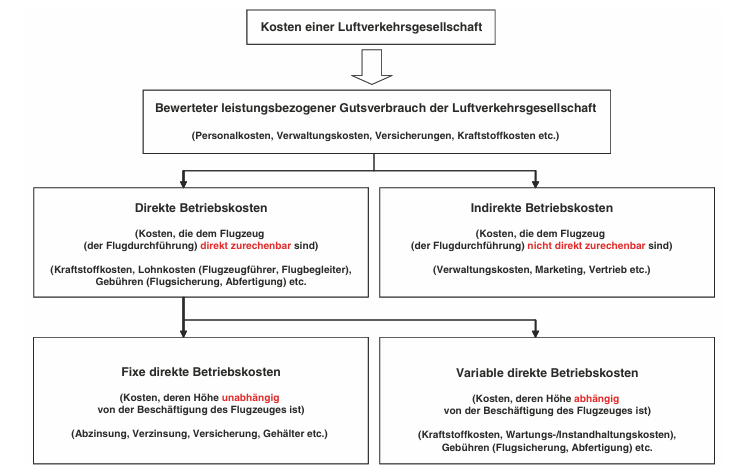
\includegraphics[width=0.9\linewidth]{Bilder/Systematik der DOC_Berechnung.png}
	\caption[DOC]{ \cite{mensen2013handbuch}}
	\label{doc}
\end{figure}


Betriebskosten sind von dem Flugzeug abhängig, deswegen ist es wichtig vor der Anschaffung zu überprüfen, 
ob es ein Flugzeug mit alternativem Antrieb rentabel ist. Die neuen Regularien für \ce{CO2}-Reduktion können einen Anreiz oder sogar 
eine Verpflichtung für die Fluggesellschaften schaffen, um die beste Lösung für eine Flotte zu finden. Mehr um politische Anreize gibt es im Kapital.

Fuel, Technikkosten (Wartung, Reparatur, Instandhaltung MRO) - es gibt unterschiedliche Typen von Wartung, die Kontrolle was am Vorfeld bei einem 
Turnaround passiert ist die line maintenance (prüfung von Reifendruck und Ölständen), Flughafenentgelte und Handlingkosten: 
Bodenabfertigung besteht aus Passagierabfertigung, Fracht-, Gepäckabfertigung und VorfelddiensteFlugzeugabfertigung ist direkte Kosten, 
Passagierkosten indirekte Kosten, Kapital- und Abschreibungskosten \cite{conrady2019luftverkehr}. 
Conrady bescheibt die Cockpit Crew als auch Cabin Crew, so Gehälter, Reisekosten, Schulungskosten. Es gibt jedoch nur wenige Arbeiten, 
die die Ausbildungskosten erwähnen. Auch Handling Agents Kosten gibt es nicht viel Information zu finden. Es kann damit zurückgeführt werden, dass
sind unabhängige von Fluggesellschaften Handling Agents für Abfertigung zuständig und nicht die Fluggesellschaften Kosten dafür übernehmen.

92 Milliarden Gallonen Kraftstoff wurden durch der Luftfahrindustrie im Jahr 2023 verbraucht.\cite{iata_industry_statistics_2024}
Kesorinpreis im Jahr 2022 betrug USD 136/bbl (ca. 133€/bbl Wechelkurs 14.01.25 \cite{ecb_exchange_rates_usd}
Der Treibstoffrechnung war fast 32\% alles Betriebskosten in der Luftfahrt im Jahr 2023. \cite{iata_industry_statistics_2024}

Wartungskosten sind von Auslastung eines Flugzeugs, je schnellere Wartung man braucht, desto teurere Komponente man braucht.

Die Kurzstrecken-Flugzeuge sind mehr mit größerer Anzahl an Landungsgebühren und größere Treibstoffverbrauch verbunden sind, da 
der Start und die Landung sind die Treibstoff aufwendigste Prozesse im ganzen Flug.

Für Szenarien Flottenabhängigkeit: Je mehr die gleichen Flugzeuge-Typen, desto geringere Wartungskosten zu erwarten.


In den USA ein Drittel von allen Gesamtkosten (TOC) aller Fluggesellschaften sind die Kosten für Treibstoff und Öl 
und ein Sechstel ist die Abfertigung am Flughafen \cite{conrady2019luftverkehr}. 

%Eine Reihe anderen Kosten, die für die Arbeit vielleicht nicht relevant?: Flugsicherungsgebühren, Versicherungskosten (bleiben), 
%Servicekosten, Marketing- und Vertriebskosten, Kpsten der allgemeinen Verwaltung, 
Diese werden aufgrund der Komplexität der Berechnungen und der begrenzten Verfügbarkeit von Daten nicht weiter betrachtet.
Cockpit crew and cabin crew Kosten bestehen aus Gehälter, Reisekosten und Schulungskosten \cite{conrady2019luftverkehr}.

"Zu den direktenvariablenKosten (flugereignisabhängige Kosten) zählen– Abfertigungsentgelte Fluggerät,– Landeentgelte,
– Flugsicherungsgebühren,– Dritthaftpflichtversicherung,– Treibstoff,– Bordservicekosten,– Reisekosten Cockpit/Kabine,
– variableInstandhaltungskosten,– variableFrachtkosten (z.B. für Anlieferung) und– Charterkosten."

"Die direkten Fixkosten (Kapazitätsvorhaltungskosten) umfassen– direktefixeTechnikkosten,– Stationswartung,
– Kapitalkosten Fluggerät,– Leasingkosten Fluggerät,– Zinsen Fluggerät,– Vorlaufkosten Fluggerät,– Versicherungen Fluggerät,
– Personalkosten Cockpit/Kabine und– Trainings-/Vorlaufkosten Cockpit/Kabine."


In den USA ein Drittel von allen Gesamtkosten (TOC) aller Fluggesellschaften sind die Kosten für Treibstoff und Öl 
und ein Sechstel ist die Abfertigung am Flughafen \cite{conrady2019luftverkehr}. 

In dieser Arbeit wird der Fokus auf die direkten Betriebskosten gemacht.




Preis für Treibstoffversorgung für kurzfristige Perioden kann folgend berechnet werden \cite{iata_saf_procurement_2024}: nicht sicher, ob die Formel nehme
PRA-Bewertung (Risikobewertung??? Durchschnitt der Vorperiode) + Logistikkosten + zusätzliche Gebühren + Lieferantenmarge


"Das Schulungsprogramm muss eine Kompetenzschulung für alle installierten Geräte umfassen." (ICAO Annex 6 Teil 2)

(Annex  Doc 1984 Teil 1 Chapter 13 Seite 141)
Bei konventionellen Kraftstoff kann die Logistik mit einem Schiff, Binnenschiff, Bahn, Lkw oder Pipeline durchgeführt. 
Diese Optionen haben große Auswirkungen auf die Kapitalkosten eines Flughafens und müssen sorgfältig berechnet werden. 
eine von spezialen Anforderungen bei Planung von Flughafeninfrastruktur "Minimierung der Belegungszeiten am Flugzeuggate; 
die erforderlichen Kraftstoffdurchflussraten sind ein Faktor bei der Wahl des einzusetzenden Betankungssystems"

Abhängigkeit der Betriebskosten von Treibstoff-Kosten beschreiben.


Abschreibungskosten sind ein Teil der Kapitalkosten für das Flugzeug, die für den festgelegten Zeitraum, wo Flugzeug benutzt wird, verteilt.


%Conceptual_Design_and_Operating_Costs_Evaluation_of_a_19-seat_All-Electric_Aircraft_for_Regional_Aviation
"die Zins- und Abschreibungskosten sinken tendenziell bei hoher Tagesauslastung"
20 Prozent in Motorwartung verringert DOC um 4%


DMC are the maintenance costs caused directly by the aircraft; 
Wartung "line maintenance cost;
periodic maintenance cost;
workshop direct maintenance cost; and
overhaul cost."

\subsection{Infrastrukturkosten}

%\subsection{Wasserstoff-Antrieb}

In vielen Forschungsarbeiten wird der Wasserstoff als die Lösung für umweltfreundliche Luftfahrt dargestellt.
Diese Alternative ist jedoch von Kosten, Sicherheit und öffentliche Akzeptanz behindert \cite{ansell2023review}.
Durch Nutzung von Wasserstoff werden keine \ce{CO2}-Emissionen verursacht, 
jedoch es können andere Abgase wie Stickoxid \ce{NOx} bei der Verbrennung in Wasserstoffturbinen oder Wasserdampf emittiert werden, 
was zur Bildung der Kondensstreifen führt(Quelle).

Zündungstemperatur?

\begin{table}[h]
	\begin{center}
    \caption{Vergleich von unkomprimiertem Wasserstoffgas hinsichtlich energiebezogenen Eigenschaften mit anderen marktüblichen Treibstoffen bei 26 \acs{Celsius} }
	\label{wasserstoff_energie}
	\begin{tabular}{|l|c|c|}
		\hline
		& \textbf{volumetrische Energiedichte in \acs{kWh/l}} & \textbf{gravimetrische Energiedichte in \acs{kWh/kg}} & \textbf{Zündungstemperatur in \acs{kWh/kg}} \\ \hline
		Wasserstoff & 2,6 \cite{colpan2022fuel} & 37,0 {colpan2022fuel} \\ \hline
		Kerosin & ~9,5 {colpan2022fuel} & ~11.9 {colpan2022fuel} \\ \hline
		 &  &  \\ \hline
	\end{tabular}
    \end{center}
\end{table}

In der Tabelle sind die Vergleichwerte für Kerosin und Wasserstoff im unterschiedlichen Zuständen. Der LH2 hat bessere Gewichtverhältnisse
als Kerosin, jedoch für die gleiche Menge Energie wird viel mehr Platz gebraucht. (flüssiger Wasserstoff - geringere Gesamtspeichermasse
-größere Flugzeuge und volumenanforderungen; für kleinere regionale - GH2)

Für die Flugzeuge ist Tankisolierung von großerer Bedeutung. Die LH2 muss bei -273 gelagert werden, ansonsten wird es zur Gas.
Das kann die Abfertigungszeiten beeinflussen. (bei schlechte Isolierung - schneller starten, bei guten - mehr Flexibilität)

Es gibt unterschiedliche Wege, um Wasserstoff zu produzieren. 
Die gängigsten Herstellungswege sind die Steam Methane Reforming (SMR) (Fully Renewable) und Elektrolyse (Fully Renewable). 
Bei SMR trifft der Wasserdampf in der Reaktion zusammen mit Methan aus Erdgas, infolgedessen entstehen 
der Wasserstoff \ce{H2} und Kohlenmonoxid bzw. -dioxid \cite{mulder2019outlook}. Elektrolyse spaltet das Wasser mithilfe von Elektrizität 
in Wasserstoff und Sauerstoff \ce{O2} \cite{mulder2019outlook}, durch dieser Herstellungsweg können CO2 Emissionen 
vollständig vermieden werden \cite{dalmia2022powering}. 

Die Nachhaltigkeit der Elektrolyse ist von der Stromquelle abhängig. 
Wenn für die Produktion vom Wasserstoff sind die erneuerbaren Energiequellen (wie Solar- und Windanlagen) benutzt worden, 
dann bezeichnet es als grüner Wasserstoff \cite{mulder2019outlook}. Wird der Strom aus fossilen Energieträger erzeugt, kommt es zu indirekten
Kohlenstoffemissionen.
Durch Elektrolyse produzierte grüner Wasserstoff ist kostenintensiv \cite{dalmia2022powering} und von der Stromkosten abhängig. 
Chardonnet et al. schätzt die 
Investitionskosten für die Produktion in 15 Mio. € (nach \cite{mulder2019outlook}).

Die Kosten für erneurbare Energie?

\cite{mulder2019outlook} - Annahme: anstatt Windkraftanlage - Stromnetz

Bei der anderen Herstellungswege (grauer und blauer Wasserstoff)
kommt es hingegen zum Ausstoß von Kohlenstoff, wobei bei blauem Wasserstoff werden die gesammelt und gespeichert \cite{mulder2019outlook}.


Wasserstoff kann in zwei unterschiedlichen Weisen als Antrieb benutzt werden: 
erstens als Treibstoff für die Verbrennung in H2-Verbrennungsmotor,
zweitens als Brennstoffzelle für elektrischen Motor anzupowern \cite{sky2020hydrogen}.

"Die Wasserstofftriebwerke werden in ihrer Architektur den bestehenden Düsentriebwerken ähneln, 
jedoch mit einigen Ergänzungen, wie z. B. Kraftstoffpumpen und -steuergeräten, Brennkammern und
 einem zusätzlichen Wärmetauscher zur Verdampfung von flüssigem Wasserstoff (LH2)" \cite{colpan2022fuel}



Flüssiger Wasserstoff

"LH2 hat die höchste spezifische Energie- und Kühlleistung aller herkömmlichen Substanzen." \cite{ansell2023review}
Flüssiger Wasserstoff entsteht durch die Verflüssigung aus H2.

Senkt man die Temperatur von Wasserstoff bis -253 °C \cite{colpan2022fuel}, entsteht flüssiger Treibstoff .

Nutzung von Wassertreibstoff ist für größere Flugzeuge geeignet und somit für längere Stecken. Das vorhergeht von 
Gewichtsanteil von LH2 Tank in Anhängigkeit von der gelagerten Menge. 
Große Flugzeuge liefern bessere Speichereffizienz und Wasserstoffmenge-Verhältnis.
"(da niedrige Tankgewichte erforderlich sind, um den hohen spezifischen Energievorteil von Wasserstoffkraftstoff voll auszuschöpfen)"
\cite{ansell2023review}


Gasförmige Wasserstoff/ Brennstoffzellentechnologie

Eine andere Methode, um Wasserstoff in der Luftfahrt zu benutzen ist der Wasserstoff im gasförmigen Zustand. 
Diese Technologie wird noch Brennstoffzellentechnologie genannt.
Durch chemische Reaktion aus gasförmige Wasserstoff \ce{H2} und Sauerstoff \ce{O2} wird Strom produziert \cite{dalmia2022powering} und 
dadurch der Propeller von dem Flugzeug angetrieben.
Brennstoffzellen (wie Polymerelektrolytbrennstoffzelle) haben größere Energiedichte (als was?) und 
können somit für die Mittel- oder Langstrecken benutzt werden \cite{dalmia2022powering}. 
Um mehr Energiedichte speichern zu können, muss \ce{H2} stark komprimiert werden.

hydrogen-Electric Antrieb

Sobald die Brennstoffzellen in das Flugzeug integriert sind, werden Generatoren/Generatoren das 
Auxiliary Power Unit (APU)-System des Flugzeugs mit Strom versorgen. Zum Einsatz kommen Brennstoffzellen 
mit Protonenaustauschmembran, deren Strom die Motoren antreibt. Die Motoren werden über Propeller verfügen,
die dann dem Flugzeug Schub verleihen, da sie sich mit unterschiedlichen Geschwindigkeiten im Verhältnis zur Drosselklappe drehen.\cite{dalmia2022powering}

Wasserstoff kann in einer chemischen Verbindung gebunden werden, wie Ammoniak und Methanol, und somit auch transportiert.

not sure:

Die Infrastruktur und Logistik ist ein wichtiger Teil der Produktionskette. Gerade wird Wasserstoff durch die Pipelines 
transportiert \cite{mulder2019outlook}. Der Transport ist durch Pipelines im gasförmigen Zustand, LKW und Zügen sowohl im gasförmigen,
als auch im flüssigen Zustand möglich. 
Transport von LH2 erfordert speziell konstruierte Tanks \cite{mulder2019outlook}
Mulder et al. schätzt die Investitionskosten für Wasserstoff durch Elektrolyse deutlicher günstiger als ein Kohlekraftwerk. 
Obwohl die hohen Kapitalkosten von Pipelines Anlage zu erwarten, sind die Betriebskosten niedrig. Also bei größeren Umfang lohnt es Pipelines, sonst Lkw


\cite{dahal2021techno} In der Dahal et el. Studie wurde ein Konzept vorgeschlagen, wo die Tanks auf dem Fuselage sich befinden.
"Die kryogenen Kraftstofftanks erfordern eine angemessene Isolierung sowie die Verwendung von Materialien, die 
gegen Versprödung und zyklische Belastungen schützen, die durch die thermische Ausdehnung und Kontraktion beim Nachfüllen 
und den Kraftstoffverbrauch verursacht werden"

Wasserstoff kann in Hochdrucktanks und Salzkavernen gelagert werden \cite{mulder2019outlook}

Die zusätzliche Ausbildung für Wartungsmitarbeiter und die Schulungen für Bodenabfertigen
werden benötigt, weil die Charakteristiken von Wasserstoff 
sich von herkömmlichen Treibstoffen stark unterscheiden.

Betriebsleergewicht bleibt konstant, im Betracht Startbruttogewicht um 30 \%, jedoch wegen großen Wasserstofftank


\section{Flugzeuge und Annahmen}
\subsection{Relevante Flugzeugdaten}
Um den betrieblichen Unterschied zwischen konventionellen und mit neuartigen Antrieben zu zeigen, werden die Referenz-Flugzeuge mit neuen 
Konzepten verglichen.
Für den Vergleich mit BA wurde für L410 entschieden. L410 ist ein Zubringer-Flugzeug mit 19 Plätzen der Firma Aircraft Industries. 
Die moderne Version L410NG verfügt über neue Avionik und mit zwei GE H85-200 Triebwerken mit einer Wellenleistung von 850 (SHP) ausgestattet.

Die ES-19 von Heart Aerospace dient als Vergleich zur L410. Das Konzept hat einen rein elektrischen, batteriebetriebenen Antrieb.
Das Unternehmen hat zwar die ES-19 auf eine hybride Wasserstoffversion ES-30 umgerüstet, das Konzept der ES-19 wurde allerdings breit diskutiert 
und oft in wissenschaftlichen Arbeiten erwähnt. Sie hat vier Triebwerke und sollte über eine Reichweite von 400 km verfügen, 
wobei sie hierbei mit einer Reisegeschwindigkeit von 330 km/h fliegt \cite{anker2023feasibility} \cite{heart_aerospace_es19}.
Für die Batterie der ES-19 wird eine Kapazität von 900 kWh angenommen \cite{donckers2024electric}. \\
Verbrauch von einem L410 beträgt 240 kg/h \cite{let2016l410}.
In der Tabelle \ref{Flugzeuge} sind relevante charakteristische Werte und Annahmen von beiden Flugzeugen zusammengefasst.
Die ES-19 ist langsamer als eine L410, d.h. das für gleiche Strecke mehr Zeit benötigt wird, was am Ende die Auslastung verändern kann.
Aufgrund des Batteriegewichts ist das BA Flugzeug schwerer als konventionelle Alternativen.

Die A321LR ist eine von Airbus vorgestellte neue Version der A321neo mit einer größeren Reichweite.
Flugzeug ist mit ... Triebwerken ausgestattet 
Da es bis jetzt nur wenig ausgearbeitete größere Konzepte für Wasserstoff-Antrieb gibt, wird der Betriebsvergleich
auf der Basis von einer A321LR stattfinden, mit der Annahme, dass Flugzeug mit Wasserstoffturbine betrieben ist.
Im Vergleich zu konventionellen Flugzeugen werden die Wasserstoff-Flugzeuge, die für Mittelstrecken geeignet, 14 \% höheres MTOW haben 
und die Kapitalkosten für das Kurzstrecken-Flugzeug sowie Wartungskosten steigen um 7 \% und 6 \% \cite{sky2020hydrogen}. 
Diese Anteile sind zwar für Mittel- und Langstrecken Flugzeuge positiv, aber werden dennoch für diese Arbeit angenommen.

Es ist auch zu erwarten, dass die Flugzeit zwischen 5 und 15 \% aufgrund des Wasserstofftank-Gewichts zunimmt \cite{sky2020hydrogen}. 
Aus diesem Grund wurde für ein Wert von 10 \% für die Arbeit entschieden.
Der Vergleich zu SAF-Betriebskosten findet auch mit der A321LR statt. Es wird davon ausgegangen, dass der Unterschied 
nur bei Treibstoffkosten entsteht. Für die A321LR wird die Passagieranzahl von 220 und Verbrauch von 1,7 kg pro Kilometer und pro PAX angenommen \cite{fonseca2022doc}.

\begin{table}[h]
	\begin{center}
    \caption{Bewertete Flugzeuge: Werte und Annahmen}
	\label{Flugzeuge}
	\begin{tabular}{|l|c|c|c|c|c|c|}
		\hline
		 & \textbf{V} ~[\text{km/h}] & \textbf{R} ~[\text{km}] & \textbf{MTOW} ~[\text{kg}] & \textbf{EOW} ~[\text{kg}] & \textbf{PAX-Anzahl} 
		 & \textbf{Quellen} \\ \hline
		L410  & 417 & 2 570 & 7000 & 4120 & 19 & \cite{let_l410ng}\\ \hline
		ES-19 &  330 & 400 & 8618 & & 19 & \cite{anker2023feasibility} \cite{heart_aerospace_es19}\\ \hline
		A321LR & 1104 & 7400 & 97000 & & 220 & \cite{airbus_a321neo} \cite{fonseca2022doc} \\ \hline
		AZEROe Turboprop &  &  &  & 110580 & -- &\\ \hline
	\end{tabular}
    \end{center}
\end{table}

Dass die Anschaffungspreise die Betriebskosten beeinflussen, wurde bereits in 2-2 diskutiert. 
Die Tabelle \ref{Flugzeugpreise} stellt die Verkaufspreise für konventionelle Referenz-Flugzeuge dar.
Da der Verkaufspreis einer A321LR nicht zur Verfügung steht, wird auf den Listenpreis einer A321neo zurückgegriffen. 
Da sie aus einer Flugzeug-Reihe kommen, kann es davon ausgegangen werden, dass die Preise ähnlich sind.
%Die Preise für alternative Antriebe sind wegen  nicht dargestellt

\begin{table}[h]
	\begin{center}
    \caption{Flugzeugpreise}
	\label{Flugzeugpreise}
	\begin{tabular}{|l|c|c|c|}
		\hline
		 & \textbf{L410} & \textbf{A321neo}  & \textbf{Quelle}  \\ \hline
		 Verkaufspreis ~[\text{EUR}] & 6 455 884 & 129,5 Mio &  \cite{marksel2023comparative} \cite{aerotelegraph_airbus}\\ \hline
	\end{tabular}
    \end{center}
\end{table}

\subsection{Sonstige Annahmen}
%\subsection{Annahmen für die Berechnung der Kosten}
%\label{s:Annahmen für die Berechnung der Kosten}

Auf der Grundlage der unterschiedlichen Quellen und vernünftigen Behauptungen wurde eine Reihe der Annahmen getroffen.

Die Betriebskosten werden mit Reisegeschwindigkeit ohne Beachtung von Start und Landung, wo auch mehr Energie verbraucht wird.
Batterie: Mit jetziger Leistung der Batterien wäre es unmöglich bei so einem Gewicht und der Distanz zu bleiben.
Deswegen wird es angenommen, dass die Batterien sich positiv in Gewicht/Leistung-ratio entwickeln und Kapazitätswert von 450 kWh/kg genommen.

Stromkosten von 0.1976 € per kWh werden auch als konstante angenommen \cite{eurostat_nrg_pc_205}.


Manche Studien gehen davon aus, dass die Einsparungen in der Wartungskosten von BA-Flugzeugen 10-15 \% erreichen können 
\cite{wangsness2021fremskyndet,avogadro2024demystifying}. Deswegen in dieser Arbeit wird ein Wert von 10 \% zu dem Referenzflugzeug genommen.

Es wird davon ausgegangen, dass Sicherheitsradius beim Wasserstoffbetankung wird nicht erweitert. 
%Diese Daten in der Literatur sind noch nicht verfügbar.

Infrastrukturkosten

Da sich die Flughäfen Position topografisch unterscheidet, wird die Annahme getroffen, dass die Lieferung mit LKW stattfindet 
und die Lieferkosten sind bereits in dem Preis von flüssigem Wasserstoff inbegriffen.

Alle Werte in USD werden mit dem Wechselkurs \footnote{Wechselkurs vom 14.01.2025} (EUR 1 = USD 1.0245) umgerechnet und beim Pfund (1,20 = EUR 1).

%Nach AEA wird die Versicherung als einem Wert von 0,5 \%  des Flugzeugpreises berechnet und durchschnittliche Verzinsungsrate ca.5 \%

%\cite{scholz_design_evaluation_doc}.
%Die Lebensdauer mach AEA für Kurz- und Mittelstrecken erreicht 14 Jahre und für die Langstrecken 16 Jahre \cite{scholz_design_evaluation_doc}.

%Beechcraft ist mit 2 Triebwerken PT6A-67D ausgestattet, Take-off power (5 Min) - 954 kW, sonst die Leistung 906 kW.\cite{easa_tcds_pt6a67}

Obwohl die maximalen Geschwindigkeiten unter Referenz- und BA-Flugzeugen sich unterscheiden werden, 
für die Kurzstrecken-Flügen ergibt es sich nicht eine sehr große Differenz.
Deswegen es wird angenommen, dass die batteriebetriebenen Flugzeuge ähnliche Auslastung wie konventionelle Flugzeuge aufweisen.

%Lebensdauer von 1000 Zyklen bis die Kapazität bis 80 \% reduziert wird für eine Li-Ion-Batterie wird angenommen, da folgende Werte bei Auto-Industrie bekannt für.
In der Zukunft ist die Lebensdauer einer Batterie bis 5000 und mehr Zyklen zu erwarten \cite{reimers2018introduction}, deswegen wurde auch dieser
Wert in der Berechnung angenommen.

Aufgrund der hohen Unsicherheit der Preisprojektionen wird der Preis für Kerosin konstant gehalten, nämlich im Wert von
0,688 EUR pro Liter \cite{iata_industry_statistics_2024}. 


%Kosten für den Markt?
%Kosten für SAF (HEFA) (Produktionskosten) Jahr 2030 - Durchschnittspreis 1.0 USD/l, 
%minimal 0.8 USD/l, 1.2 USD/l. 
%Fossil jet range with CO2 price 0.4-0.9 USD/l für Jahr 2021 (Carbon price = USD 50/tonne.)\cite{iea_biojet_2021}
In Anbetracht der Kostensenkung für nachhaltige Kraftstoffe in der Zukunft, wird der minimale Preis für HEFA-Treibstoff 
von 1,07 EUR pro Liter wird in den Rechnungen verwendet \cite{watson2024sustainable}.

Lieferkosten für flüssigen Wasserstoff und HEFA werden nicht explizit ausgerechnet,
da die schon in Betriebskosten von Wasserstoff-getriebene Flugzeuge eingeschlossen sind. Es wird vor allem angenommen, dass die Produktion 
des Wasserstoffes und Verflüssigung nicht am Flughafen stattfindet, sondern eingekauft und zum Flughafen transportiert.

Es wird angenommen, dass die Batterien für BA zur Flughafen-Infrastruktur gehören, 
d.h. die Anschaffungskosten Flughafen anfallen und danach werden die für Fluggesellschaften ausgeliehen.
Die Inflationsfaktoren stammen aus Verbraucherpreisindex Deutschland aus Statistischem Bundesamt.

Die Besatzungskosten sind mit Lohn von 37 EUR für Flugbegleiter und 90 EUR für Piloten pro Blockstunden berechnet \cite{discover_airlines_cabin}.

Die konstante Spitzenleistung von Batteriewechselsystem von 250 kW wird angenommen. Der Strom ist normalerweise von Tag und Nacht abhängig
und wie viel parallel genutzt wird. Angenommen ist die Batteriekapazität, wie bei der ES-19, dauert es 3,6 h bis die Batterie geladen wird.
d.h. 10 fzg jeder braucht batterie, dann diese batterie kann erst in 4 std benutzt werden.

\section{Aufstellung der Formeln für Kosten}
\label{s:Aufstellung der Formeln für Kosten}

Wie bereits im Kapitel 2 beschrieben wurde, werden die Kosten einer Fluggesellschaft auf direkte und indirekte Betriebskosten verteilt.
In diesem Kapitel werden die dazugehörigen Formeln vorgestellt und teilweise angepasst. 

Es gibt eine Reihe von Methoden, um DOC zu berechnen, wobei diese oft ähnlich sind.
Als Grundlage für ein Modell wurde %hier fehlt das modell oder?
der Association of European Airlines (AEA) 1989 gewählt, da sie häufige Anwendung in der akademischen Welt hat,
sehr umfassend ist und Berechnungswerte für sowohl Kurz-, als auch Langstecken hat.

Der Reservebedarf beträgt 30 \% der Gesamtkapazität.



\subsection{Betriebskosten einer Fluggesellschaft}

Die Gleichung \eqref{DOC} stellt die Betriebskosten $DOC$ der Flugzeugnutzung dar. Diese bestehen aus Treibstoff-/Energiekosten $C_T$, 
Wartungskosten $C_W$, Entgelten und Gebühren $C_{EG}$, Kosten für Personal $C_{Crew}$ und kapitalgebundenen Kosten $C_{KK}$.


\begin{equation}
     {DOC ~[\text{EUR}]} = C_T + C_W + C_{Crew} + C_{KK} + C_{EG} \\
     \label{DOC}
  \end{equation}

\textbf{Treibstoff-/ Energiepreise} hängen vom Treibstoff- bzw. Energiepreis selbst \\ $P_{T/E}$ und vom Verbrauch 
eines Flugzeugs pro Blockstunde $m_{Verbrauch_pro_Flug}$ ab (vgl. \eqref{fuel}).



\begin{equation}
   {C_T ~[\text{EUR}]} = (P_{T/E} \cdot n_{F,Jahr} \cdot m_{Verbrauch,B}) \\
   \label{fuel}
\end{equation}

Die \textbf{Wartungskosten} werden nach dem Jenkinson 1999 Modell berechnet. Das Modell ermöglicht es, grob aber schnell die Wartungskosten 
für ein Flugzeug abzuschätzen \cite{bruge2018wartungskosten}.
Da dieses Modell auf konventionelle Flugzeuge ausgearbeitet wurde, berechnet man die Wartungskosten für alternative Antriebe
als Prozentanteil des Referenz-Flugzeugs. 
Die Formeln stammen aus \cite{bruge2018wartungskosten} und beziehen sich auf das Jahr 1994, somit muss der Inflationsfaktor $k_{Infl}$
einkalkuliert werden. Die Berechnung liefert die Ergebnisse in USD, aus diesem Grund wird ein Wechselkursfaktor $k_{WK}$ in die Berechnung implementiert.
Wartungskosten werden normalerweise auf die Wartung der Flugzeugzelle $C_{W,Zelle,B}$ und der Triebwerke 
$C_{W,Triebwerk,B}$ aufgeteilt, wie in Gleichung \eqref{maintenance} dargestellt. Die Wartungskosten der Zelle sind von dem leeren Betriebsgewicht 
(Operating Empty Mass $m_{OE}$) abhängig. Kosten des Triebwerks sind vom erzeugten Schub beim Start (Take-Off Thrust $T_{T/O}$) abhängig.

\begin{equation}
   {C_{W,B} ~[\text{EUR}]} = (C_{W,Zelle,B} + n_{T} \cdot C_{W,Triebwerk,B} ) t_{B} \cdot n_{F, Jahr} \cdot k_{WK} \cdot k_{Infl}\\
   \label{maintenance}
\end{equation}

\begin{equation}
   {C_{M,AF,b} ~[\text{EUR}]} = (175 \frac{USD}{h} + 0,0041 \frac{USD}{h} \cdot m_{OE} )\cdot k_{Infl}\\
   \label{maintenance Zelle}
\end{equation}

\begin{equation}
   {C_{M,E,L,b} ~[\text{EUR}]} = (0,00029 \frac{USD}{h} \cdot T_{T/O} )\cdot k_{Infl}\\
   \label{maintenance engine}
\end{equation}

Diese Formeln sind für Triebwerke mit Nebenstromverhältnis ausgelegt 5. %warum hier die 5?
Trotz der höheren Nebenstromverhältnisse die bei moderneren und größeren Flugzeugen gegeben sind,
wird aus Gründen der Vereinfachung trotzdem diese Formel genutzt.

%Wartungskosten wachsen mit der Größe des Flugzeugs, da mehr Personal oder mehr Zeit für die Wartung benötigt ist.

Unter \textbf{Entgelte und Gebühren} sind Flughafenentgelte (Passagier-, Lande- und Startentgelte, Sicherheitsentgelte sowie Abfertigung am 
Vorfeld) und die Flugsicherungsgebühr gemeint. 
Die Formel der Flugsicherungsgebühr $(C_{FS})$ für jeweils An- und Abfluggebühr stammt aus \cite{dfs_flugsicherungsgebuehren} und ist in der Gleichung \eqref{Flugsicherung}
dargestellt. Im Jahr 2025 liegt der Wert $P_{FS}$ bei 380,71 Euro. 
Der $MTOW$ bezeichnet das Höchstabfluggewicht (Maximum Take-Off Weight) eines Flugzeugs. 
Die zugrunde liegenden Werte der Flughafenentgelte basieren auf den Daten von \cite{fraport2025entgelte}.
Außerdem müssen bei BA-Flugzeugen die Kosten für
Batteriewechsel $P_{W,Bat}$ einkalkuliert werden, pro Flugzeug wird ein Wert von einem Wert in Höhe von 285 EUR ausgegangen \cite{guo2023infrastructure}.

\begin{equation}
   {C_{FS} ~[\text{EUR}]} = (\frac{MTOW}{50})^{0,7} \cdot P_{FS} \\
   \label{Flugsicherung}
\end{equation}

Die Betriebskosten werden auf Basis von Blockstunden kalkuliert. 
Blockstunden setzen sich aus Flugzeit $t_{F,h}$ sowie der kumulierten Rollzeit $t_{R}$ von und zur Parkposition $t_{R}$ zusammen. 
Für Kurz- und Mittelstrecken beträgt $t_{R}$ {0,25 h} und für Langstrecken 0,42 h \cite{scholz_design_evaluation_doc}.

\begin{equation}
   t_{B} = t_{f,h,j} + t_{R} \\
   \label{blockzeit}
\end{equation}

\textbf{Crewkosten} setzen sich aus Lohnkosten für Piloten $L_{Pilot}$ und Besatzung $L_{crew}$ zusammen. Die Anzahl der Besatzungmitglieder $n_{crew}$ ist 
von der Anzahl der Passagiere abhängig. Gemäß den luftfahrtrechtlichen Bestimmungen ist pro 50 Passagiere ein Flugbegleiter notwendig \cite{conrady2019luftverkehr}.

\begin{equation}
   {C_{crew} ~[\text{EUR}]} = ({L}_{Pilot} \cdot 2 + {L}_{crew} \cdot n_{crew} ) \cdot t_{B} \\
   \label{crew cost}
\end{equation}

%Der Preis für ganzes Flugzeug außer Antrieb-System wird nach folgend berechnet

%\begin{equation}
%   {P_{i,f} ~[\text{€}]} = \frac{m_{i,f}}{m_{i,c}} \cdot p_{i,c} \cdot P_{A,C} \\
%   \label{aicraft price hydrogen}
%\end{equation}



 
%Analog zum \cite{marksel2023comparative} werden die Kosten für den Wasserstoff und Batterie Antrieb getrennt ausgerechnet, 
%wobei für Batterie-Antrieb anstatt eines Wasserstofftanks und eine Brennstoffzelle, basiert sich auf einer Batterie, Motor 
%und Leistungselektronik

%\begin{equation}
%   {P_{E,f} ~[\text{€}]} = P_{FC} \cdot + P_{EM} \cdot + m_F \\
%   \label{engine group price hydrogen}
%\end{equation}
Zu \textbf{kapitalbezogenen Kosten} gehören Abschreibungs-, Versicherungs- und Verzinsungskosten. 
Abschreibungskosten sind von Anschaffungskosten (Kaufpreis), Abschreibungsdauer und Blockstunden pro Jahr abhängig \cite{conrady2019luftverkehr}.
Die Abschreibungsdauer nach AEA beträgt jeweils 14 Jahre für Kurz- und Mittelstecken und 16 Jahre für Langstrecken.

Da keine öffentlich zugänglichen Marktpreise für Luftfahrzeuge mit alternativen Antriebssystemen vorliegen, 
wird die Kalkulation der Anschaffungskosten für elektrisch betriebene Flugzeuge nach der Methodik von \cite{monjon2020conceptual} durchgeführt, 
in welcher das Regressionsmodell anhand einer Marktanalyse erstellt wurde. 
In der Formel sind aufgrund der Einführung neuer Technologien 10 \% höhere Anschaffungskosten mitbetrachtet. 
Die Studie ist aus dem Jahr 2020, Preise wurden in USD berechnet, weshalb die Inflationsrate $k_{Infl}$ 1,193 und
der Wechselkurs $k_{WK}$ ebenfalls betrachtet werden sollen.

\begin{equation}
   {C_{BA,ac} ~[\text{EUR}]} = (407408 \cdot n_{PAX} - 2967.4) \cdot k_{WK} \cdot {k_{Infl}}\\
   \label{price BA}
\end{equation}

<<<<<<< HEAD
Noch ein wichtiger Faktor bei der kapitalverbundenen Kosten ist die Auslastung $U$ eines Flugzeuges. Es wird durch Anzahl 
verfügbaren Stunden pro Jahr $t_{verf}$, Blockzeit $t_B$ und Turnaround Zeit $t_{TA}$. $t_{verf}$ für Kurzstrecken wurde 
in der Höhe von 3750 h und für Mittel- und Langstrecken 4800 h \cite{scholz_design_evaluation_doc}. $t_{TA}$ wurde in Höhe von 1,5
Stunden gewählt (Quelle).
=======
Ein weiterer wichtiger Faktor der kapitalgebundenen Kosten ist die Auslastung $U$ eines Flugzeuges. Es wird durch die Anzahl 
der verfügbaren Stunden p.a. $t_{verf}$, Blockzeit $t_B$ und Turnaround Zeit $t_{TA}$ berechnet. 
Die jährliche Verfügbarkeitszeit $t_{verf}$ beträgt für Kurzstreckenflugzeuge 3750 h, 
während für Mittel- und Langstreckenflugzeuge ein Wert von 4800 h angesetzt wird \cite{scholz_design_evaluation_doc}.
>>>>>>> 5f8c26e (überprüfung 1)

\begin{equation}
   U = \frac{t_{verf}}{t_B + t_{TA}} \\
   \label{utilisation}
\end{equation}

<<<<<<< HEAD
Verzinsungskosten sind durch den Prozentanteil von Anschaffungskosten bedingt, für dieser gilt ca. 5 \%. Versicherungskosten sind 
hingegen von dem Kaufpreis eines Flugzeugs abhängig (inklusive Rabatte beim Kauf) und für diese Arbeit werden 5 \% angenommen 
\cite{scholz_design_evaluation_doc}.
=======
Verzinsungskosten $C_{Zins}$ sind durch den Prozentanteil von Anschaffungskosten bedingt, für diese gelten ca. 5 \%. 
Versicherungskosten sind hingegen von dem Kaufpreis eines Flugzeugs abhängig (inklusive Rabatte beim Kauf), 
in dieser Arbeit werden ebenfalls 5 \% angenommen \cite{scholz_design_evaluation_doc}.
>>>>>>> 5f8c26e (überprüfung 1)

%Für wasserstoffbetriebene Flugzeuge werden in der Quelle vorgestellte Formeln benutzt, um Kaufpreis einschätzen zu können.
Außerdem bestehen bei alternativen Antrieben betriebliche Kosten, die durch Infrastrukturbedienung bedingt sind.
\subsection{Infrastrukturkosten}

\textbf{Batterie-Antrieb}\\
Kapitalkosten für BA-Infrastruktur sind in folgender Formel zusammengestellt:

\begin{equation}
     {CAPEX ~[\text{EUR}]} = C_{Bat} + C_{Strom} + C_{BSS} + C_{W,Bat} + C_{Hubwagen}\\
     \label{BA_Infrastruktur}
  \end{equation}

\begin{equation}
   \begin{split}
  {C_{Bat}} = P_{Bat} \cdot n_{Bat}\\
  {C_{Strom}} = n_{BSS} \cdot P_{Strom} \cdot N_{menge}\\
  {C_{BSS}} = P_{BSS} \cdot n_{BSS} \\
  %(\frac{30}{Lebensdauer})\\
  {C_{Hubwagen}} = P_{Hubwagen} \cdot n_{Hubwagen}
  \label{BA}
   \end{split}
  \end{equation}

<<<<<<< HEAD
, wobei $P_{Bat}$ ist der Preis für eine Batterie und $n_{Bat}$ ist der Anzahl Batterien, die benötigt sind.
$N_{menge}$ ist die Menge an Strom, der für das Laden einer Batterie benötigt ist.
$P_{BSS}$ ist der Preis für Ladegerät der Batteriewechselstation und $n_{BSS}$ ist wie immer der Anzahl an Ladegeräten. 
Zusätzlich werden die Kosten für
Batteriewechsel $P_{W,Bat}$ und Preis für einen Hubwagen $P_{Hubwagen}$ mitbetrachtet.
  
%Energiekosten = Menge mal Preis

 % Stromkosten = Anzahl der BSS mal die Leistung mal Kosten pro Einheit Spitzleistung mal Anzahl der Tage/30

  %Anschaffungskosten BSS = Anzahl BSS mal Kosten mal Tage/Lebensdauer
=======
wobei $P_{Bat}$ der Preis für eine Batterie darstellt und $n_{Bat}$ die Anzahl der Batterien, die benötigt sind.
$N_{menge}$ ist die Menge an Strom, der für das Laden einer Batterie nötig ist.
$P_{BSS}$ ist der Preis des Ladegeräts der Batteriewechselstation und $n_{BSS}$ ist wie immer der Anzahl an Ladegeräten. %ich weiß nicht was du mit wie immer meinst
Außerdem werden die Kosten für Batteriewechsel $P_{W,Bat}$ und Preis pro Hubwagen $P_{Hubwagen}$ mitbetrachtet.
  
%Energiekosten = Menge mal Preis

Stromkosten = Anzahl der BSS mal die Leistung mal Kosten pro Einheit Spitzleistung mal Anzahl der Tage/30

Anschaffungskosten BSS = Anzahl BSS mal Kosten mal Tage/Lebensdauer
>>>>>>> 5f8c26e (überprüfung 1)

 % An Optimization Model for Airport Infrastructures in Support to Electric Aicraft:
 % Um Batterienachfrage zu decken, wäre es möglich der Anzahl der Ersatz-Batterien zu erhöhen, die außerhalb der Spitzzeiten geladen werden 
 % oder der Anzahl der Batteriewechselstationen zu erhöhen. Es wird angenommen, dass für Flughafen 800 kW - Ladestationen zur Verfügung haben, 
 % (Studie, wo die Leistungen für
 % 3 hybride-Flugzeuge ausgerechnet wurden - insgesamt für 12 Flugzeuge sind 21 Batterien und 4 Ladestationen benötigt, 77,5 € pro Station, Peak power 3,2 MW, Batteriewechsel jede 1.51 Jahre
 % also eine Station für 3 Flugzeuge?). Natürlich in der Zukunft werden die Flugzeuge unterschiedliche Leistungen
 % und auch Batterien brauchen, was am Ende die Ladedauer und Anzahl der Ladestationen ändern kann

%10 \% für die Wartung der Systeme (wie bei OPTIMAL RECHARGING INFRASTRUCTURE SIZING AND OPERATIONS 
%FOR A REGIONAL AIRPORT)


\begin{table}[h]
	\begin{center}
    \caption{Werte und Annahmen der BA-Infrastruktur}
	\label{BA_Infrastrukturtab}
	\begin{tabular}{|l|c|c|}
		\hline
		 & \textbf{Werte} & \textbf{Quelle} \\ \hline
		$P_{BSS} ~[\text{EUR}]$ &  11 974  & \cite{guo2020aviation} \\ \hline
		$P_{Bat} ~[\text{EUR/kWh}]$ & 125000 & \cite{guo2020aviation} \\ \hline
		$P_{W,Bat} ~[\text{EUR}] $ & 285  & \cite{guo2023infrastructure}\\ \hline
      $P_{HW} ~[\text{EUR}] $ &  &\\ \hline
	\end{tabular}
    \end{center}
\end{table}

Die Anzahl der Batterien ist von der Gesamtanzahl der Abfertigungen $N_{Abfertigung}$ und Zyklen $c_{Batterie}$ einer Batterie abhängig. 
Für die Ladegeräte wurde die Leistung von 250 kW angenommen. 
Die Verluste beim Laden werden ignoriert. 
Zusätzlich wird der Puffer von 20 \% implementiert, um Engpässe zu vermeiden. 
In dieser Arbeit wird eine Batteriekapazität von 900 kWh angenommen, bei einem 18 Stunden-Betrieb 
entspricht das 3,6 Stunden Ladedauer für eine Batterie mit insgesamt 5 Ladezyklen pro Tag. 
Die Anzahl der Ladegeräte $n_{BSS}$ ist von der Gesamtzahl der Batterien und Ladezyklen abhängig.

\begin{equation}
  {N_{Bat}} = {1,2} \cdot \frac{N_{Abfertigung}}{c_{Batterie}}\\
  \label{BatAnzahl}
  \end{equation}

\textbf{Wasserstoff-Antrieb}

%Lieferung
%falls in flüssigform: LKW/Schiff/Bahn - Distanz und von der Menge abhängig.

<<<<<<< HEAD
Für die Wasserstoff-Antriebe wird einen oberirdischen Tank für kryogene flüssigen Wasserstoff \ce{LH2}, eine kryogene Pumpe 
zum Befüllen und Entleeren des Lagers ${kP}$ und ein Betankungswagen ${BW}$ gebraucht (vgl. \eqref{WA_Infrastruktur}). 
Die Preise für die Anlage ist in der Tabelle \ref{BA_Infrastrukturtab} aufgeführt. Es werden zwei Pumpensysteme benötigt.
Eine davon ist zum Befüllen des Betankungswagens an den \ce{LH2}-Speicher und andere beim Betanken des Flugzeuges \cite{hoelzen2022h2}.
=======
Für Wasserstoff-Antriebe wird ein oberirdischer Tank für kryogenen flüssigen Wasserstoff \ce{LH2}, 
eine kryogene Pumpe zum Befüllen und Entleeren des Lagers ${kP}$ und ein Tankwagen ${BW}$ gebraucht (vgl. \eqref{WA_Infrastruktur}). 
Die Preise für die Anlage sind in der Tabelle \ref{BA_Infrastrukturtab} zusammengefasst.
>>>>>>> 5f8c26e (überprüfung 1)

\begin{equation}
   {CAPEX ~[\text{EUR}]} = {P_{Tank}} + P_{kP} + P_{BW} \cdot N_{BW}  \\
   \label{WA_Infrastruktur}
\end{equation}

\begin{table}[h]
	\begin{center}
    \caption{Werte und Annahmen}
	\label{BA_Infrastrukturtab}
	\begin{tabular}{|l|c|c|c|}
		\hline
		 & \textbf{Werte}& \textbf{Einheit}& \textbf{Quellen} \\ \hline
		$P_{Lagertank}$ & 34 & EUR/kgGH2 stored  & sek \cite{hoelzen2023h2}\\ \hline
      Abschreibung Lagertank & 20  & Jahre  & sek \cite{hoelzen2023h2}\\ \hline
      Größe Lagertank ~[\text{$m^3$}] & 4 732 &  & \cite{fesmire2021lh2}\\ \hline
		$P_{kP}$ & 346 & EUR/kg/h & sek \cite{hoelzen2023h2} \\ \hline
      Abschreibung ${kP}$ & 10 & Jahre & sek \cite{hoelzen2023h2} \\ \hline
		$P_{BW}$ & 87848 & EUR & \cite{hoelzen2022h2} \\ \hline
	\end{tabular}
    \end{center}
\end{table}

<<<<<<< HEAD
Wie bereits in Grundlagen-Kapitel erläutert wurde, hat den kryogenen Wasserstoff die Dichte von 70 $kg/m^3$ (Quelle), 
also können 331,24 t davon in einem kugelförmigen Lagertank gespeichert werden.
Es wird davon ausgegangen, dass die Vorgänge der Betankung des Wagens und folgende Betankung des Flugzeugs jeweils 
30 Minuten dauern \cite{hoelzen2022h2}. (1 Flugzeug pro Tankwagen, also alles von - Ankunftsrate abhängig)



=======
Wie bereits im Grundlagen-Kapitel erläutert wurde, hat der kryogene Wasserstoff eine Dichte von 70 $kg/m^3$ (Quelle),  %quelle?
also können 331.240 t in einem Lagertank gespeichert werden.
>>>>>>> 5f8c26e (überprüfung 1)


\section{Betriebsszenarien}
\label{s:Betriebsszenarien}
Betriebsszenarien helfen die vorher beschriebenen Betriebs- und Infrastrukturkosten in Anwendung zu bringen 
und eine mögliche Entwicklung in der nahen Zukunft aufzuzeigen. 
Die Größe des Flughafens beeinflusst die Infrastrukturkosten. 
Bei einem größeren Flughafen werden die Betriebsdifferenzen deutlicher, da das Verkehrsaufkommen wesentlich höher ist.
Größere Flughäfen fertigen täglich mehr Flugzeuge als Regionalflughäfen ab, 
was dazu führt, dass mehr Abfertigungsplätze umgerüstet und versorgt werden müssen,
wodurch mehr Arbeitskräfte geschult werden müssen.

Deshalb wird für die Betriebsszenarien der Flughafen Frankfurt gewählt,
welcher als bedeutendes Luftverkehrsdrehkreuz fungiert
und zudem der größte Verkehrsflughafen Deutschlands ist.
Der Fraport meldete im Jahr 2023 insgesamt 423764 gewerbliche Flugbewegungen, was im Durchschnitt 1160 Flugbewegungen pro Tag ausmacht. 
Es wird angenommen, dass die Hälfte davon Abflüge sind, also müssen 580 Flugzeuge pro Tag abgefertigt werden.
%
Die Gesamtbewegungen teilen sich nach Entfernungen folgend auf \cite{fraport2023frankfurt}:
\begin{itemize}
    \item Kurzstrecken (bis 2500 km) sind bei 72,8 \%;
    \item Mittelstrecken (bis 6000 km) sind 9,3 \%;
    \item Langstrecken (ab 6000 km) die restlichen 17,9 \%. 
    \end{itemize}
Da nicht explizit definiert wird, welche Entfernungen die Flugzeuge zurücklegen, werden die Betriebskosten anhand vorher beschriebener Distanzen berechnet.
Dabei wird für Kurzstrecken eine Entfernung von 400 km und für Langstrecken eine Distanz von 6000 km angenommen.
Für Mittelstrecken werden die selben Werte wie bei Langstreckenflügen verwendet, jedoch mit einer anderen Distanz von 4000 Kilometer,
dass Treibstoffverbrauch pro Stunde sich nicht ändern wird.

Anhand der zugrundeliegenden Informationen wird eine Flotte mit 580 Flugzeugen aufgestellt, in welcher alternative Antriebe eingesetzt werden.
Aufgrund der Flugeinschränkungen in der Nacht wird angenommen, dass die Flüge von 6 bis 24 Uhr gleichmäßig stattfinden. 
Wie bereits diskutiert wurde, können Kurzstrecken-Flüge durch den Einsatz von batteriebetriebenen Flugzeugen ersetzt werden, 
wobei hier als Ersatz auf SAF zurückgegriffen wird. Es ist nennenswert, dass nur ein Teil der tatsächlichen Nachfrage des Kurzstrecken-Bedarfs 
dadurch gedeckt werden kann. Die Mittel- und Langstrecken werden von Flugzeugen mit Wasserstoffturbine und SAF durchgeführt.
%
Durch Betrachtung des tatsächlichen Flugplans sind die Spitzenstunden eines Tages zu ermitteln, bei welchen Verkehrsfluss stärker als im Durschschnitt ist.
In diesem Fall werden höhere Infrastruktur- und Betriebskosten erwarten zu sein.
Um die Interpretation zu erleichtern, wird in dieser Arbeit angenommen, dass stündlich die gleiche Anzahl an Flugzeugen 
am Flughafen abgewickelt werden. 
%
Die Aufteilung der Antriebe für jedes Szenario ist in der Abbildung \ref{betriebsszenarien} dargestellt.
%
\begin{figure}[h]
	\centering
	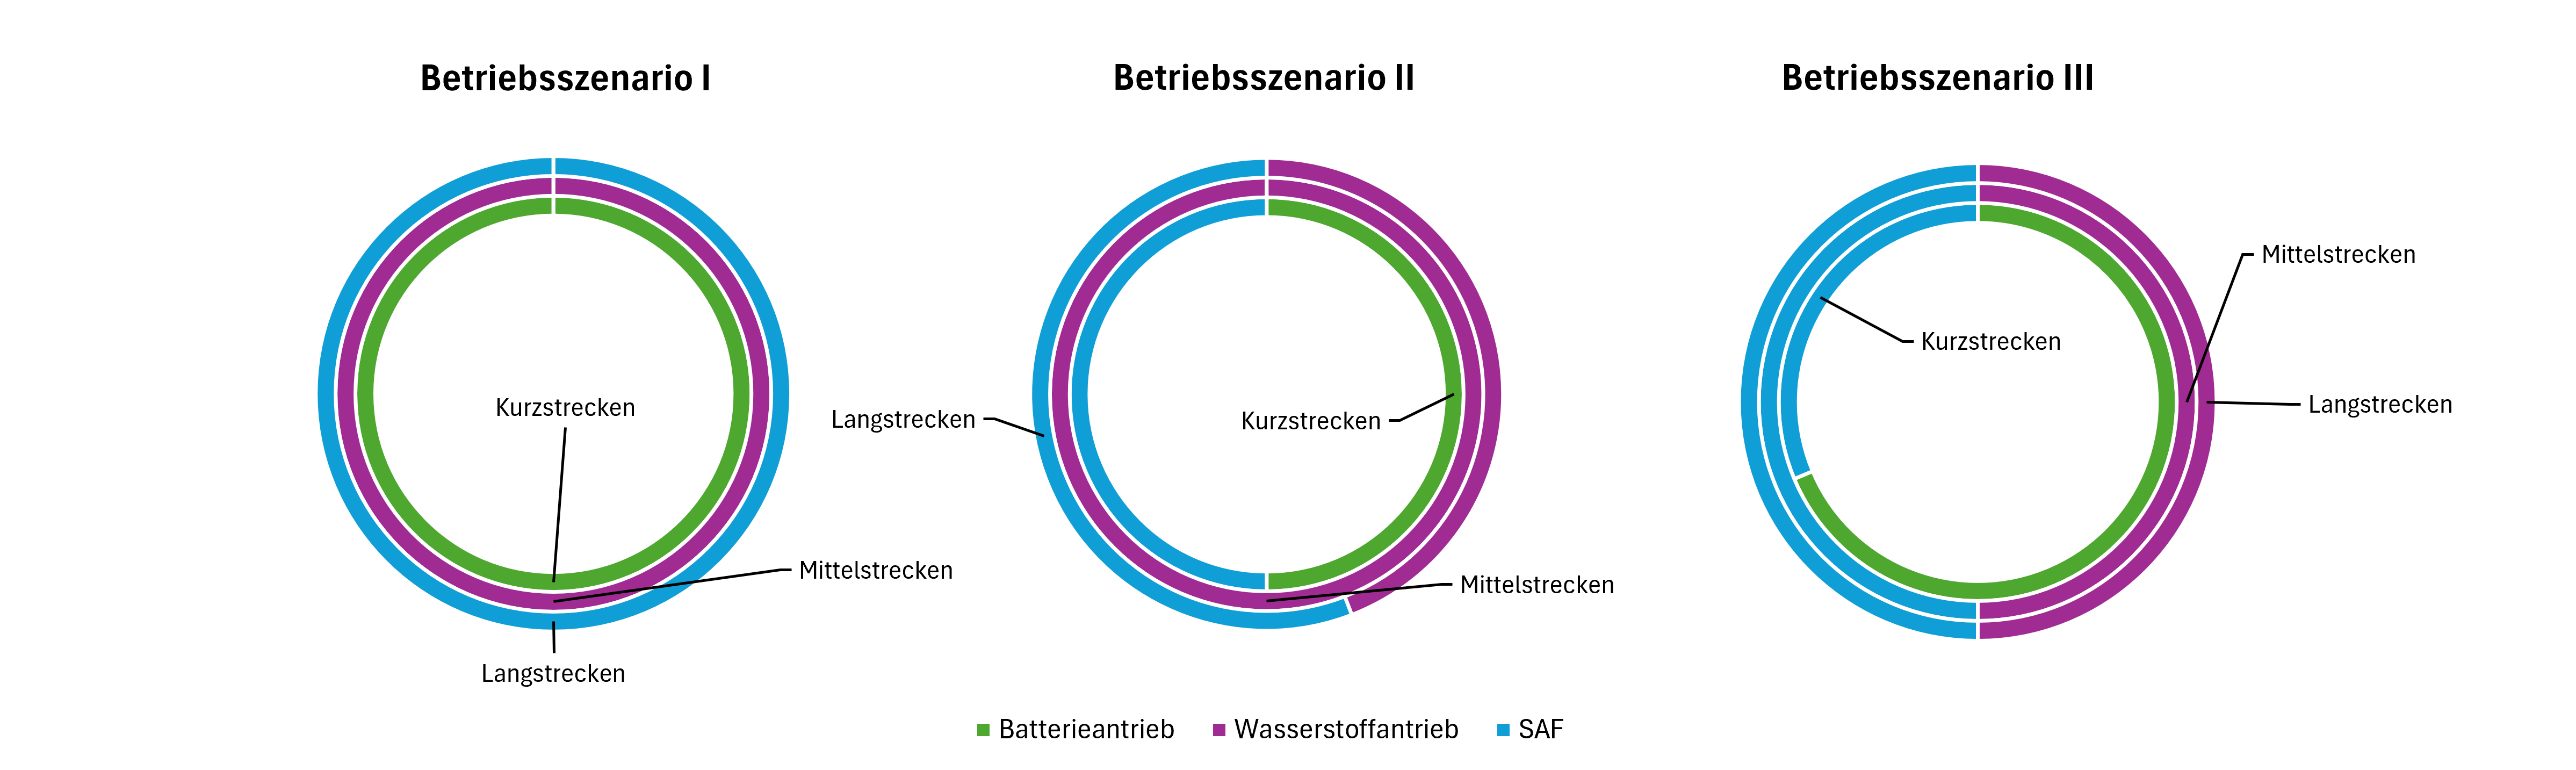
\includegraphics[width=1.0\linewidth]{Bilder/Betriebsszenarien.png}
	\caption[Betriebsszenarien]{Aufteilung der Flugzeugflotte nach Antriebsart}
	\label{betriebsszenarien}
\end{figure}
%
In dem \textbf{ersten Betriebsszenario} wird angenommen, dass:
\begin{itemize}
    \item Die Kurzstrecken durch den BA komplett ersetzt werden;
    \item Die Mittelstrecken werden vollkommen durch WA und
    \item die Langstrecken durch SAF bedient.
\end{itemize}
Das \textbf{zweite Betriebsszenario} wird mit folgender Aufteilung berechnet:
\begin{itemize}
    \item 50 \% der Kurzstrecken wird durch BA und 50 \% durch SAF betrieben; 
    \item die Mittelstrecken werden, genau wie im ersten Szenario, komplett durch Wasserstoffflugzeuge betrieben und 
    \item Langstrecken werden zu 10 \% der Gesamtflotte durch SAF und der Rest durch Wasserstoff bedient.
\end{itemize}
Das \textbf{dritte Szenario}:
\begin{itemize}
    \item 50 \% der Kurzstrecken werden durch BA, die restlichen 22,8 \% mit SAF betrieben
    \item Mittelstrecken: 50 \% der Mittelstrecken werden mit WA und 50 \% mit SAF betrieben
    \item Langstrecken: 50 \% der Langstrecken werden mit WA und die 50 \% mit SAF betrieben
\end{itemize}
%
Daraus ergibt sich die folgende Flottenaufteilung für die einzelnen Szenarien:
\begin{table}[h]
	\begin{center}
    \caption{Werte und Annahmen der BA-Infrastruktur}
	\label{BA_Infrastrukturtab}
	\begin{tabular}{|c|c|c|>{\centering\arraybackslash}p{3cm}|c|}
		\hline
		\multicolumn{4}{|c|}{\textbf{Szenario I}} \\ \hline
		 & \textbf{Batterieantrieb} & \textbf{Wasserstoffantrieb} & \textbf{SAF} \\ \hline
		Kurzstrecken & 422 & - &-\\ \hline
      	Mittelstrecken & -  & 54 &- \\ \hline
		Langstrecken & - & - &104 \\ \hline
		\multicolumn{4}{|c|}{\textbf{Szenario II}} \\ \hline
		Kurzstrecken & 211 &- &211\\ \hline
      	Mittelstrecken &  - & 54 &- \\ \hline
		Langstrecken &- & 46  &58 \\ \hline
		\multicolumn{4}{|c|}{\textbf{Szenario III}} \\ \hline
		Kurzstrecken & 290 &- &132\\ \hline
      	Mittelstrecken &  - & 27 & 27 \\ \hline
		Langstrecken &  -& 52 &52 \\ \hline
	\end{tabular}
    \end{center}
\end{table}

%\documentclass[11pt]{article}
%\usepackage{cite}

%\begin{document}

%\title{Bibtex}

%\maketitle

%jzjzjz \cite{conrady2019luftverkehr}

%\bibliography{Quellen.bib}
%\bibliographystyle{plain}
%\end{document}

\phantomsection\addcontentsline{toc}{chapter}{Literaturverzeichnis}
% Einbinden der Bibliothek

% cite everything in the bib with:
\nocite{*}

{
	\small % reduces fontsize
	\printbibliography
	\normalsize % resets fontsize back to normal
}



\end{document}
